% !TeX encoding = UTF-8
% !TeX program = xelatex
% !TeX spellcheck = en_US

\documentclass[degree=bachelor]{ustcthesis}
% degree      = doctor | master | bachelor
% degree-type = academic | professional | engineering
% language    = chinese | english
% fontset     = windows | mac | ubuntu | fandol

% 加载宏包、全部的配置
\input{ustcsetup}


\begin{document}


\ustcsetup{
    title={基于生成式先验的人像视频编辑},
    title*={Portrait Video Editing Based on Generative Prior},
    author={汪兆辰},
    student-id={PB21010362},
    speciality={信息与计算科学},
    supervisor={张举勇}
}
\maketitle
% \copyrightpage

\frontmatter
\include{chapters/innovations}  % 博士学位论文的创新性说明
% !TeX root = ../main.tex

\ustcsetup{
  keywords  = {学位论文, 摘要, 关键词},
  keywords* = {Dissertation, Abstract, Keywords},
}

\begin{abstract}
  随着数字媒体技术的飞速发展和短视频平台的普及,视频内容创作已成为互联网时代的重要表达方式。
  其中,肖像视频编辑作为视频处理领域的核心应用之一,在影视制作、社交媒体、虚拟现实等领域具有广泛需求。
  传统的生成式人工智能视频编辑方法主要依赖于2D图像处理技术,难以满足3D场景下的高质量、高效率编辑需求。

  在这一背景下,PortraitGen系统代表了当前肖像视频编辑技术的前沿水平。该系统通过将2D肖像视频编辑问题
  提升至3D领域,利用动态3D高斯场确保空间和时间一致性,并创新性地引入神经高斯纹理机制,实现了高质量、
  高效率的多模态肖像视频编辑。
  
  本文基于PortraitGen算法设计并实现了一个完整的视频编辑系统,采用前后端分离的系统架构,开发了完整的
  用户工作流,并实现了管理员监控系统,以支持用户的行为分析和数据监控。

\end{abstract}

\begin{abstract*}
  With the rapid development of digital media technology and the widespread adoption of short 
  video platforms, video content creation has become an essential mode of expression in the 
  internet era. Among these, portrait video editing, as one of the core applications in video 
  processing, holds extensive demand in fields such as film production, social media, and virtual 
  reality. Traditional AIGC video editing methods primarily rely on 2D image 
  processing techniques, making it difficult to meet the requirements for high-quality and 
  high-efficiency editing in 3D scenarios.

  Against this backdrop, the PortraitGen system represents the cutting edge of current portrait 
  video editing technology. By elevating the 2D portrait video editing problem into the 3D domain, 
  the system employs a dynamic 3D Gaussian field to ensure spatial and temporal consistency while 
  innovatively introducing a Neural Gaussian Texture mechanism, thereby achieving high-quality, 
  efficient, and multimodal portrait video editing.

  This paper designs and implements a comprehensive video editing system based on the PortraitGen 
  algorithm. Adopting a frontend-backend decoupled architecture, the system develops a complete 
  user workflow and implements an administrator monitoring system to support user behavior 
  analysis and data monitoring.
\end{abstract*}

\tableofcontents
% \listoffigures
% \listoftables
\listoffiguresandtables
% \include{chapters/notation}

\mainmatter
% !TeX root = ../main.tex

\chapter{引言}

\section{研究背景与意义}

\subsection{研究背景}

随着人工智能技术的快速发展和5G网络的全面普及,全球数字内容产业正在经历前所未有的变革。
根据国家广电总局最新发布的《中国网络视听发展研究报告(2025)》显示,中国网络视听用户规模
已达10.91亿,其中短视频用户规模突破10.40亿,日均使用时长高达156分钟,稳居各类互联网应用之首。
这一庞大的用户基数和旺盛的内容创作需求,对视频编辑技术提出了更高要求,特别是在实时性、
智能化和个性化方面。

当前,AI视频编辑技术已成为行业关注的焦点。以PortraitGen为代表的先进算法已能实现100FPS的高效渲染,
支持文本、图像驱动的多模态编辑;Live2Diff采用单向的时间注意力机制,能够以近乎实时的速度将实时视频流
转换为风格化内容;ChatAnyone等风格化肖像视频生成模型的发展也十分迅速。然而,这些前沿算法在实际应用
中仍面临着诸多挑战,由于缺乏完善的用户交互
设计,限制了其广泛推广和应用,提高了前沿技术的使用门槛;另外,因为没有直接面向用户,研究者往往无法了解
用户的真实需求与体验反馈。

\subsection{研究意义}

本研究基于PortraitGen算法,构建了一套完整的智能视频编辑系统。我们设计了直观的用户界面与用户工作流,使
用户无需关心算法细节,即可轻松实现视频在文字、图像等多模态输入下的风格化处理、虚拟合成、背景光重构等功能。
同时,我们搭建了管理员系统,使研究者可以通过用户反馈和操作日志,了解用户的使用情况,从而根据用户的真实需求
优化算法,调整研究方向。

本文的主要贡献包括:
\begin{itemize}
    \item 提出面向生产环境的PortraitGen工程化方案,实现算法到产品的完整转化
    \item 设计了可扩展的用户工作流,可以搭载多种算法,实现各种算法的切换
    \item 通过实际应用验证,为行业提供可复制的技术方案
\end{itemize}

\section{论文结构}

本文的组织结构如下:
\begin{itemize}
    \item \textbf{引言}:介绍研究的背景与意义
    \item \textbf{相关工作}:详细讨论PortraitGen技术原理、现有视频编辑App的现状以及技术栈选择;
    \item \textbf{系统设计}:介绍系统的整体架构、前端设计、后端设计、数据库设计及安全性设计;
    \item \textbf{功能实现}:详细描述用户管理、视频编辑功能及管理员功能的实现细节;
    \item \textbf{性能评估}:通过功能测试、性能测试及用户体验评估,验证系统的有效性和稳定性;
    \item \textbf{改进与展望}:提出系统改进方向和未来工作展望;
    \item \textbf{结论}:总结本文的研究成果,强调本文的贡献及未来展望。
\end{itemize}


\include{chapters/floats}
\include{chapters/math}
\include{chapters/citations}

\bibliography{bib/ustc}  % 参考文献使用 BibTeX 编译
% \printbibliography       % 参考文献使用 BibLaTeX 编译

\appendix
% !TeX root = ../main.tex

\chapter{补充材料}


\section{系统运行展示}

为了更直观地说明系统的运行情况,我们在这里通过运行截图辅以文字说明的方式来进行展示。

\subsection{用户管理展示}

进入系统后自动跳转至dashboard路由,对应系统的主面板,如\ref{append:dashboard}所示。

\begin{figure}[ht]
    \centering
    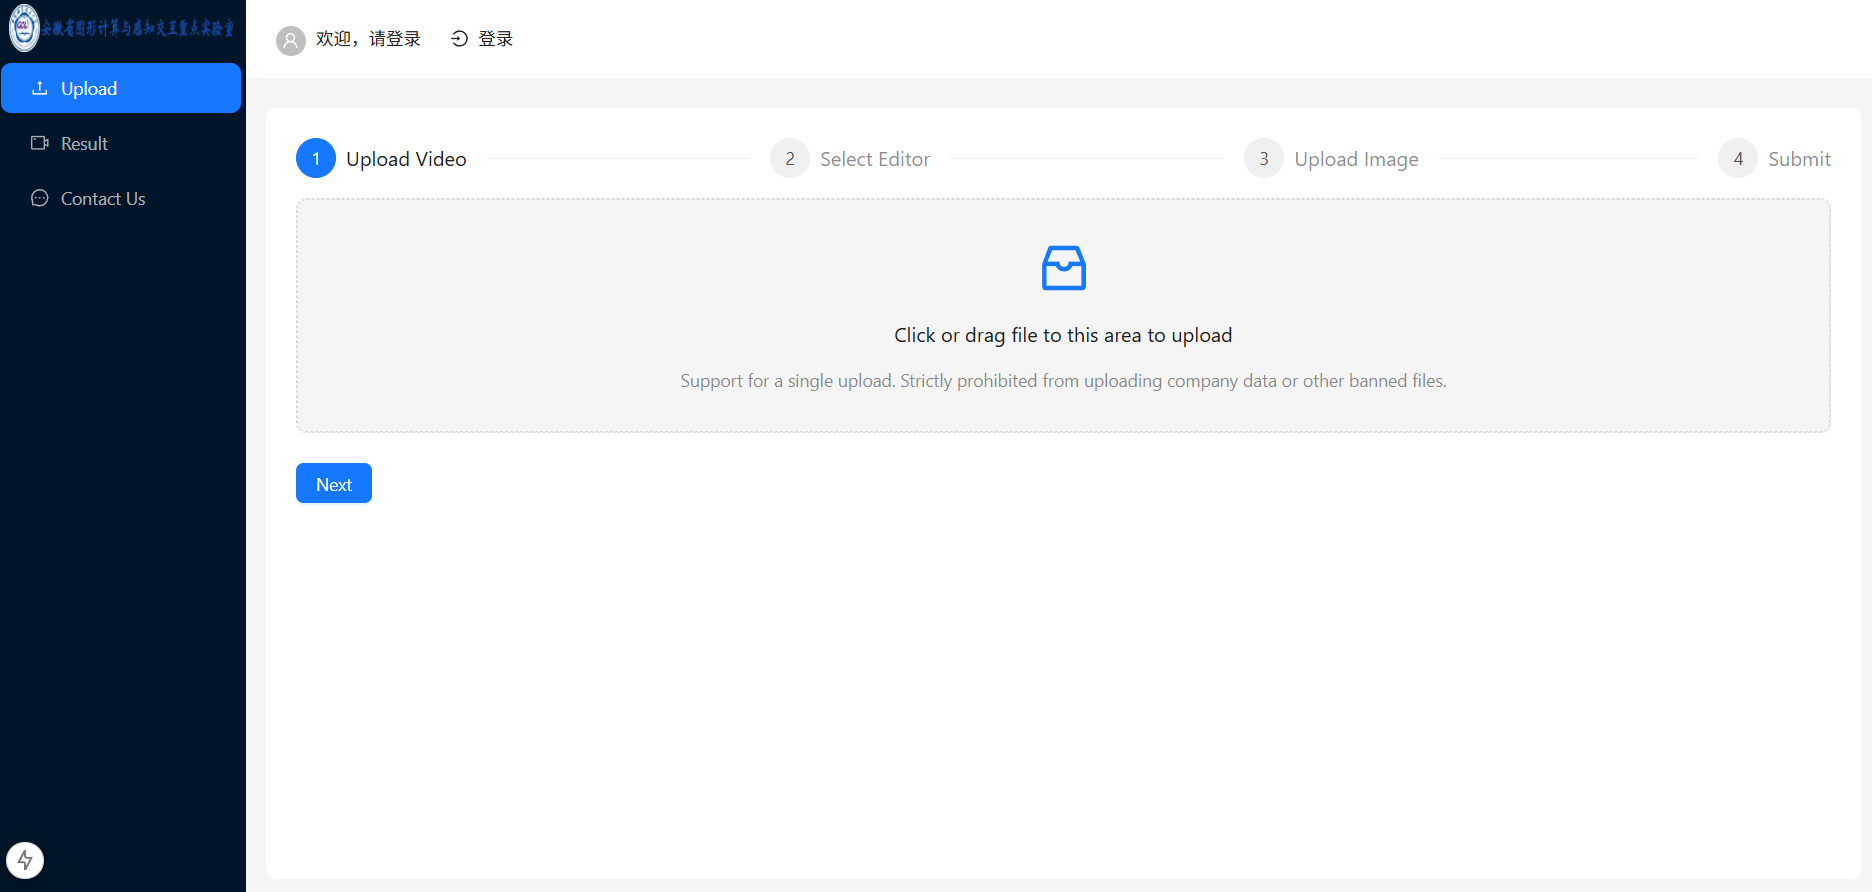
\includegraphics[width=0.8\textwidth]{source/append/dashboard.png}
    \caption{系统主界面}
    \label{append:dashboard}
\end{figure}


\backmatter
% !TeX root = ../main.tex

\begin{acknowledgements}

站在春日的尾声回望,庭梧新绿初展,叶叶如掌。值此论文付梓之际,才惊觉四年时光竟如春樱般翩然将逝。

首先,感谢我的父母。二十余载春秋,我在你们无私的爱中长大。漫漫求学路上,你们一直给予我包容与支持,让我能够走自己想走的路,
追求自己的梦想。成为你们的孩子,是我此生最大的幸运。

感谢我的导师张举勇教授。您严谨的治学态度与睿智的学术见解,如明灯般照亮我学术探索的每一步。无论是在我的保研、留学申请,
还是在我的毕业论文撰写过程中,您都给予了我细心的指导与宝贵的帮助。您的教诲将伴随我一生,成为我不断前行的动力。

感谢实验室的郭玉东特任副研究员,高玄学长与杨圣铭学长。在我的研究遇到瓶颈时,你们给予了我无私的帮助与指导,让我能够顺利完成论文的关键部分。

感谢我的母校中国科学技术大学和数学科学学院。四年前,我怀揣着对数学的热爱和对科学的向往,踏入了这片沃土。四年的时光,我如愿学习到了
渴望的知识,结识了志同道合的朋友,也收获了宝贵的经历。即便四年后的今天我已不再坚持当年数学理论研究的梦想,我仍然不后悔来到科大数院的选择。

最后感谢这一年来陪伴在我身边的雨睿同学。琴瑟易鼓,子期难再。能在人海中与你相遇,是岁月予我最好的馈赠。

停笔之时,窗外蝉鸣渐起,方觉已然入夏。

\end{acknowledgements}

\include{chapters/achievements}

\end{document}
